\chapter{Quantum Algorithms}
For many students, practice is the best way to learn so in this chapter we study  some quantum algorithms.  
\section{Deutsch-Jozsa Algorithm}
The problem is : given a function $\textit{f} : \{0,1\}^n \rightarrow \{0,1\}$ whose definition in unknown, determine whether that function is constant or balanced, knowing for certain that $\textit{f}$ will be either constant or balanced. \\
What does it mean? Well $\textit{f}$ is just a machine that "eats" a string of length $n$ composed by 0 and 1, and spits out either a 0 or a 1, lets do and example with just 2 bits : 

\begin{center}
\begin{tabular}{|c|c|}
\hline
$\{0,1\}^2$ & \textit{f} \\
\hline
  00   & 1 \\
\hline
   01  &  1 \\
   \hline
   10 & 0 \\
   \hline
   11 & 0 \\
   \hline
\end{tabular}
\quad
\begin{tabular}{|c|c|}
\hline
$\{0,1\}^2$ & \textit{f} \\
\hline
  00   & 1 \\
\hline
   01  &  1 \\
   \hline
   10 & 1 \\
   \hline
   11 & 1 \\
   \hline
\end{tabular}   
\end{center}
In the example above each row of the tables represent a " question " asked to the oracle, we have 2 bits so $\{0,1\}^2$ is a string of length 2, the whole set is in general of dimension $2^n$ so in our case we can create four different combinations. \\
We can notice that the table on the left represents a balanced function in fact as output it gives the exact same number of 0 and 1, the table on the right represents a constant function. \\
It is easy to see that in order to be sure about the nature of our function, if we have $n$ bits,we have to ask a number of questions equal to half plus one of the size of our set : $2^{n-1} + 1$, in contrast in the quantum case we will see how we need only ask one question. \\ 
We start by implementing the algorithm for 2 qbits and then we can generalize for $n$ qbit.
\newpage
\subsection{Implementation for two qbits}
\textit{By making mistakes we learn}, we will implement the Deutsch algorithm by trial and error.
As we can see in figure \ref{Deutsh2Bits} we start with two bits both at state $\ket{0}$, since the oracle calculates \textit{f} on the first qbit, in order to maximize the potential of qbits we apply the Hadamard gate to the first qbit so that we have a state in superposition. \\
\begin{figure}[h]
    \centering
    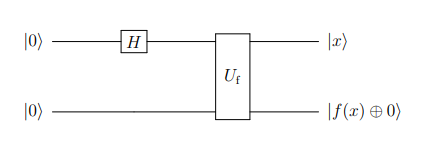
\includegraphics{QuantumAlgorithms/images/Deutsch2Bits.png}
    \caption{\todo{caption}}
    \label{Deutsh2Bits}
\end{figure}
\\
We denote the state after the i-th operation $\ket{\psi_i}$. \\
So we have the initial state : 
\begin{align*}
    \ket{\psi_1} = \ket{00} = \begin{pmatrix}1 \\ 0 \\ 0 \\ 0\end{pmatrix}
\end{align*}
After applying the hadamard gate to the first qbit we have :
\begin{align*}
    \ket{\psi_2} &= H\ket{0} \otimes \mathbb{I}\ket{0} \\[10pt]
    &= \qty(\frac{\ket{0} + \ket{1}}{\sqrt{2}})\ket{0} \\[10pt]
    &= \frac{\ket{00} + \ket{10}}{\sqrt{2}}
\end{align*}
At the end of our circuit we have : 
\begin{align*}
    \ket{\psi_3} &= \frac{\ket{0,f(0)\oplus 0} + \ket{1, f(1) \oplus 0}}{\sqrt{2}} \\[10pt]
    &= \frac{\ket{0,f(0)} + \ket{1,f(1)}}{\sqrt{2}}
\end{align*}
\newpage
Effectively our circuit calculates what we need, the problem is that the final state is kept in superposition so measuring it we would have a 50\% chance of having \textit{f(0)} and 50\% chance of having \textit{f(1)}. \\
Let's try another approach, we set the second qbit to 1 and apply hadamard gate to it, to be as general as possible the first is set to any state

\begin{figure}[h]
    \centering
    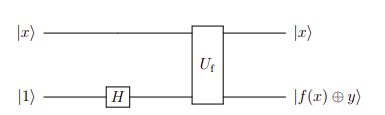
\includegraphics{QuantumAlgorithms/images/Deutsch2Bit2.png}
    \label{Deutsh2Bits2}
\end{figure}

\begin{align*}
    \ket{\psi_2} &= \ket{x} \otimes H\ket{1} \\[10pt]
                 &= \frac{\ket{x,0} - \ket{x,1}}{\sqrt{2}}
\end{align*}

\newpage
